\documentclass[../main.tex]{subfiles}

\begin{document}
\begin{enumerate}[(a)]

\item Halle el valor de la constante $k$ que permite que la función de densidad
de probabilidad de la variable aleatoria X esté correctamente definida.

$$\int_{0}^{5} \left( \frac{x^2}{50} - \frac{x}{15} + kx\right) dx = 1$$
$$\left.\frac{x^3}{150}\right\vert_{0}^{5} +  \left.\frac{x^2}{30}\right\vert_{0}^{5} + \left.\frac{kx^2}{2}\right\vert_{0}^{5}= 1 \iff 0.833 - 0.833 + 12.5k = 1 \Rightarrow k = \frac{1}{12.5}$$
$$k = 0.08$$

\item A partir del enunciado, establezca la función de probabilidad de Y dado
X.

$$f_{x}(X) = \frac{x^2}{50} - \frac{x}{15} + 0.08x \wedge R[Y] = \frac{x}{2} \leq y \leq 2x$$
$$f(Y | X) =  \frac{1}{2x - x/2} = \frac{1}{(3x)/2} = \frac{2}{3x}$$

\item Encuentre la función de densidad de probabilidad conjunta y grafique la
región en la cual se encuentra definida.

$$f(Y | X) = \frac{f(x, y)}{g(x)} \Rightarrow f(x, y) = f(Y | X) \times g(x)$$
$$f(x, y) = f(Y | X) \times g(x) = \left( \frac{2}{3x}\right) \times \left( \frac{x^2}{50} + \frac{x}{75}  \right) = \frac{x}{75} + \frac{2}{225}$$

\begin{figure}[h]
\centering
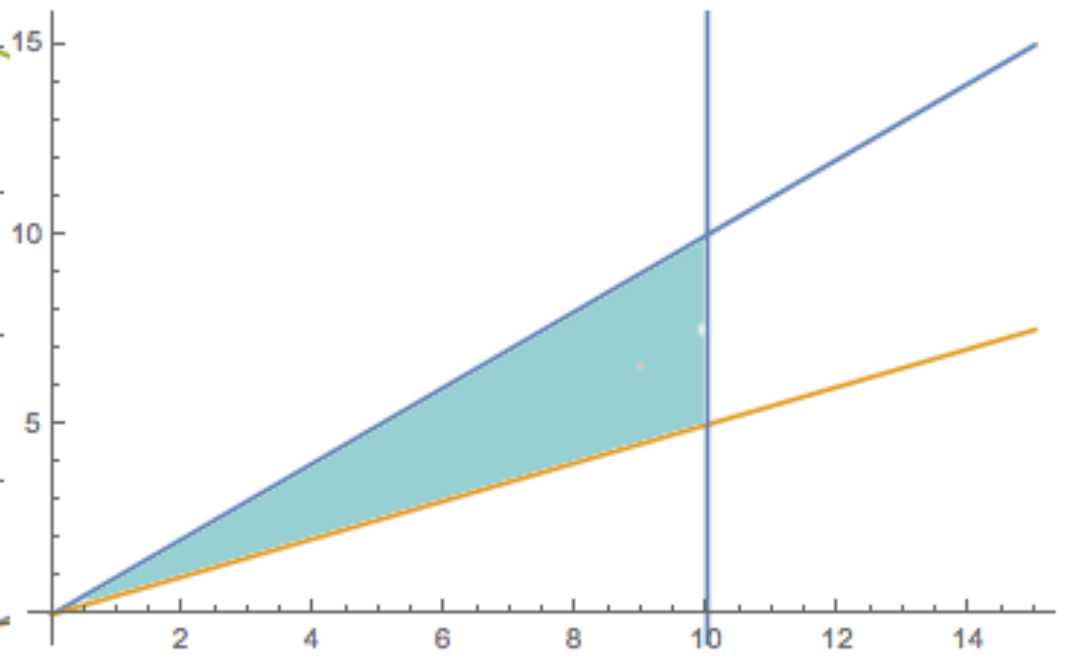
\includegraphics[width=8cm]{fig3-1}
\label{fig:img1}
\caption{Región de definición de la función de densidad conjunta}
\end{figure}

\pagebreak

\item Calcule la probabilidad de que la utilidad obtenida por la venta de
accesorios más la utilidad obtenida por la venta de computadores portátiles durante
la temporada escolar sea menor a \$4000 USD. Para esto especifique los siguientes
pasos:

\begin{enumerate}[(I)]

\item Grafique la región donde se encuentra definida la probabilidad solicitada.

\begin{figure}[h]
\centering
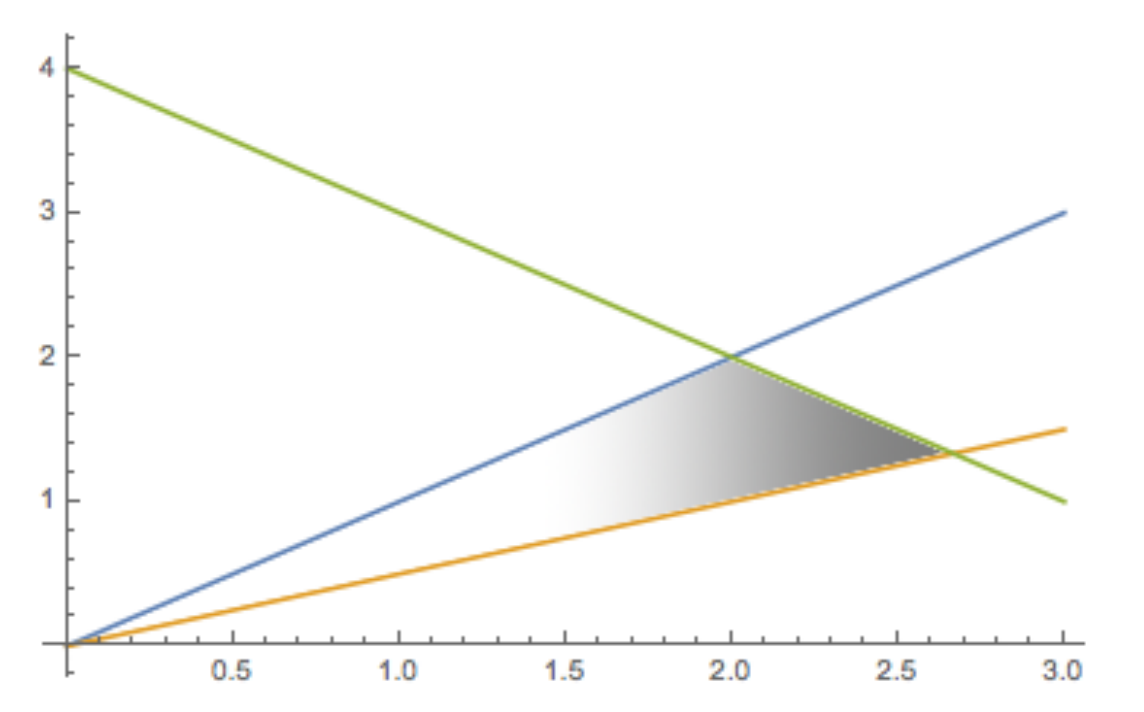
\includegraphics[width=8cm]{fig3-2}
\label{fig:img1}
\caption{Región de la probabilidad}
\end{figure}

$$4 - x = \frac{x}{2} \Rightarrow 8 - 2x = x \Rightarrow x = \frac{8}{3}$$
$$4 - x = 2x \Rightarrow x = \frac{4}{3}$$

\item Calcule la probabilidad requerida.

$$f(x, y) = 0.0133x + 0.009$$
$$\mathbb{P}_{1}(Y < 4 - X) = \int_{0}^{4/3} \int_{2x}^{x/2} \left( \frac{x}{75} + \frac{2}{225} \right) \ dx$$
$$\mathbb{P}_{1}(Y < 4 - X) =\int_{0}^{4/3} \left( \left( \left.\frac{x^2}{2(75)} + \frac{2x}{225}\right)\right\vert_{2x}^{x/2} \right) \ dx$$
$$\mathbb{P}_{1}(Y < 4 - X) =\int_{0}^{4/3} \left(\frac{4x^2}{2(75)} - \frac{x^2}{8(75)} + \frac{4x}{225} - \frac{x}{225}\right) \ dx$$
$$\mathbb{P}_{1}(Y < 4 - X) = 0.0316$$

$$\mathbb{P}_{2}(Y < 4 - X) = \int_{4/3}^{8/3} \int_{x/2}^{4-x} \left( \frac{x}{75} + \frac{2}{225} \right) \ dx$$
$$\mathbb{P}_{2}(Y < 4 - X) = \int_{4/3}^{8/3} \left( \left( \left.\frac{x^2}{2(75)} + \frac{2x}{225}\right)\right\vert_{4-x}^{x/2} \right) \ dx$$
$$\mathbb{P}_{2}(Y < 4 - X) = \int_{4/3}^{8/3} \left( \frac{16-2(4)x + x^2}{2(75)} - \frac{x^2}{8(75)} + \frac{8 - 2x}{225} - \frac{x}{225} \right) \ dx$$
$$\mathbb{P}_{2}(Y < 4 - X) = 0.0395$$
$$\mathbb{P}(Y < 4 - X) = \mathbb{P}_{1}(Y < 4 - X) + \mathbb{P}_{2}(Y < 4 - X)  = 0.0711$$
\end{enumerate}

\item Halle la función de densidad de probabilidad marginal de la variable
que representa la utilidad obtenida por la venta de accesorios.

$$h(y) = \int_{R[X]} f(x, y) \ dx$$

\[ R[X] = \begin{cases} 
      y/2 < x < 2y \\
      y/2 < x < 5
   \end{cases}
\]

$$h_{1}(y) = \int_{y/2}^{2y} \left( \frac{x}{75} + \frac{2}{225} \right) \ dx = \left. \left(\frac{x^2}{2(75)} + \frac{2x}{225}\right)\right\vert_{2y}^{y/2}$$
$$h_{1}(y) = \frac{4y^2}{2(75)} -  \frac{y^2}{8(75)} + \frac{4y}{225} - \frac{y}{225} = \frac{y^2}{40} + \frac{y}{75}$$

$$h_{2}(y) = \int_{5}^{y/2} \left( \frac{x}{75} + \frac{2}{225} \right) \ dx = \left. \left(\frac{x^2}{2(75)} + \frac{2x}{225}\right)\right\vert_{y/2}^{5}$$
$$h_{2}(y) = \frac{25}{2(75)} -  \frac{y^2}{8(75)} + \frac{2(5)}{225} - \frac{y}{225} = \frac{-y^2}{600} - \frac{y}{225} + 0.211$$

\[ h(y) = \begin{cases} 
      \frac{y^2}{40} + \frac{y}{75} & 0 < y < 5/2 \\
      \frac{-y^2}{600} - \frac{y}{225} + 0.211 & 5/2 < y < 5
   \end{cases}
\]

\item Calcule la probabilidad de que la utilidad obtenida por las ventas de
accesorios sea menor a \$4000 USD.

$$h(Y < 4) = \int_{0}^{5/2} \left( \frac{y^2}{40} + \frac{y}{75}\right) \ dy + \int_{5/2}^{4} \left( -\frac{y^2}{600} + \frac{y}{225} + 0.2111\right) \ dy = 0.439$$

\item Calcule el valor esperado de la utilidad de la venta de accesorios.
Interprete el resultado en términos del problema.

$$\mathbb{E}(y) = \int_{R_1[Y]} y \times h(y) \ dy + \int_{R_2[Y]} y \times h(y) \ dy$$
$$\mathbb{E}(y) = \int_{0}^{5/2} y \times \left( \frac{y^2}{40} + \frac{y}{75}\right) \ dy + \int_{5/2}^{4} y \times \left( -\frac{y^2}{600} + \frac{y}{225} + 0.2111\right) \ dy = 4.6$$

4600 USD se espera sea la utilidad de la venta de los accesorios.

\item Si se sabe que la utilidad obtenida por la venta de computadores
portátiles fue de \$4000 USD, calcule el valor esperado de la utilidad obtenida por
las ventas de accesorios. Interprete el resultado en términos del problema.

$$\mathbb{E}(Y | X = x) = \int_{R[Y]} \left( y \times f_{y}(y | X = x)\right) \ dy$$
$$\mathbb{E}(Y | X = 4) = \int_{0}^{10} \left( y \times \frac{2}{12}\right) \ dy = 8.33$$

\item \hl{Si se sabe que la utilidad} de portátiles está entre 2000 y 4000. ¿Cuál es
el valor esperado de la utilidad de los accesorios?

\item Determine si las variables aleatorias son independientes entre sí.

$$f(x, y) \neq h(y) \times f(x) \Rightarrow \text{No son independientes}$$

\item Calcule el coeficiente de correlación e interprete este valor en términos
del problema.

$$\rho_{XY} = \frac{Cov(X, Y)}{\sigma_{X} \times \sigma_{Y}} = \frac{\mathbb{E}(XY) - \mathbb{E}(X)\mathbb{E}(Y)}{\sigma_{X} \times \sigma_{Y}}$$
$$\rho_{XY} = \frac{\left[ \int_{0}^{5} \int_{x/2}^{2x} \left( xy \times \left( \frac{x}{75} + \frac{2}{225}\right) \ dy \ dx \right) \right] - \mathbb{E}(X)\mathbb{E}(Y)}{\sigma_{X} \times \sigma_{Y}}$$
$$\rho_{XY} = \frac{\left[ \int_{0}^{5}  \left.\left(\frac{y^2}{2}\left(\frac{x^2}{75} + \frac{2x}{225}\right)\right)\right\vert_{x/2}^{2x} \ dx  \right] - \mathbb{E}(X)\mathbb{E}(Y)}{\sigma_{X} \times \sigma_{Y}} = \frac{\left[ \frac{875}{98}  \right] - \mathbb{E}(X)\mathbb{E}(Y)}{\sigma_{X} \times \sigma_{Y}}$$

$$\mathbb{E}(X) = \int_{R[X]} x \times f_{X}(x) \ dx = \int_{0}^{5} x \times \left( \frac{x^2}{50} - \frac{x}{15} + 0.08x \right) \ dx = 3.605$$
$$\mathbb{E}(X^2) = \int_{R[X]} x^2 \times f_{X}(x) \ dx = \int_{0}^{5} x^2 \times \left( \frac{x^2}{50} - \frac{x}{15} + 0.08x \right) \ dx = 14.58$$

De manera análoga, $\mathbb{E}(Y) = 4.6$ y $\mathbb{E}(Y^2) = 25.52$.

$$\mathbb{V}ar(X) = 14.58 - (3.605^2) = 1.58$$
$$\mathbb{V}ar(X) = 25.52 - (4.6^2) = 4.36$$
$$\rho_{XY} = \frac{\left[ \frac{875}{98}  \right] - (3.605)(4.6)}{\sqrt{1.58} \times \sqrt{4.36}} = 0.63$$


\end{enumerate}
\end{document}